\documentclass[tikz,border=3.14mm]{standalone}

\begin{document}
    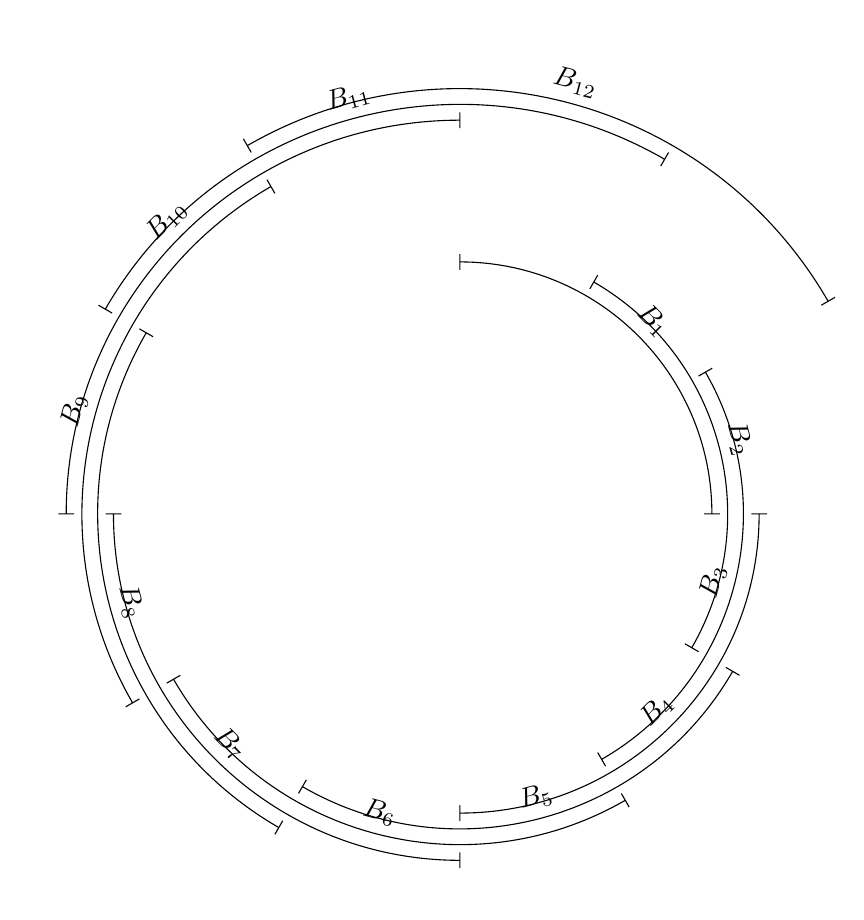
\begin{tikzpicture}
        \tikzset{declare function={hourstoangle(\h) = 90-(\h)*360/12;}}
        \def\dialR{3cm} % dial radius
        
        % dial
        %\draw (0,0) circle[radius=\dialR];
        
        % hour tips
        %\foreach \num in {1,...,12}{
            %\draw ({hourstoangle(\num)}:\dialR)-- ++({hourstoangle(\num)}:-1mm);
        %}
        
        % hour labels
        %\foreach \num in {1,...,12}{
            %\draw ({hourstoangle(\num)}:\dialR-5mm) node{\num};
        %}
        
        % arcs
        \foreach \num [count= \n from 1] in {0,...,11}{%\foreach \num in {0,...,12}{ I only need 12 and not 13 arcs
            \pgfmathsetmacro\dist{\dialR+2mm+2mm*\num}
            
            \draw
            % two tips
            ({hourstoangle(\num)}:\dist pt-1mm) -- ({hourstoangle(\num)}:\dist pt+1mm)
            ({hourstoangle(\num+3)}:\dist pt-1mm) -- ({hourstoangle(\num+3)}:\dist pt+1mm)
            % one arc
            ({hourstoangle(\num)}:\dist pt)
            arc[start angle={hourstoangle(\num)},end angle={hourstoangle(\num+3)},radius=\dist pt] node[sloped,midway,above]{$B_{\n}$};
        }
        
        
    \end{tikzpicture}

    
    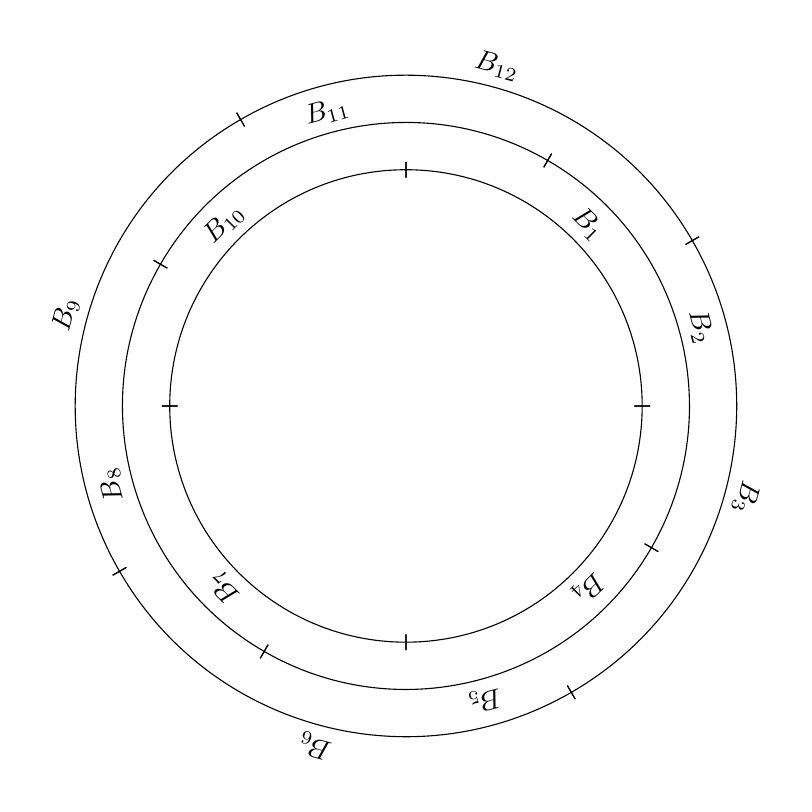
\begin{tikzpicture}
        \tikzset{declare function={hourstoangle(\h) = 90-(\h)*360/12;}}
        \def\dialR{3cm} % dial radius
        
        \newcommand{\drawcircle}[1]{
            \pgfmathsetmacro\dist{\dialR+#1 mm}
            
            \draw
            % two tips
            ({hourstoangle(\num)}:\dist pt-1mm) -- ({hourstoangle(\num)}:\dist pt+1mm)
            ({hourstoangle(\num+3)}:\dist pt-1mm) -- ({hourstoangle(\num+3)}:\dist pt+1mm)
            % one arc
            ({hourstoangle(\num)}:\dist pt)
            arc[start angle={hourstoangle(\num)},end angle={hourstoangle(\num+3)},radius=\dist pt] node[sloped,midway,above,allow upside down]{$B_{\n}$};}
        % arcs
        \foreach \num [evaluate = \num as \n using int(\num+1)] in {0,3,6,9}{%
            \drawcircle{0}
        }
        \foreach \num [evaluate = \num as \n using int(\num+1)] in {1,4,7,10}{%
            \drawcircle{6}
        }
        \foreach \num [evaluate = \num as \n using int(\num+1)] in {2,5,8,11}{%
            \drawcircle{12}
        }
       
        
        
    \end{tikzpicture}   
    
\end{document}